% Example of including an image
The first step to complete the project was to choose and understand the dataset that it needs to train the model. First of all, the dataset was fully labeled, which helps to train the model the right way and also to visualize the given data. \\~\\
To visualize the data, it was split in 2 sets, the positive and the negative ones, and then with the use of Python modules there was created at first a data frame (pandas module) and then a histogram (plotly.express module), to see how the dataset is distributed, and a matrix of images and their labels (numpy, keras.preprocessing and matplotlib.pyplot modules).
\begin{figure}[H]
    \centering
    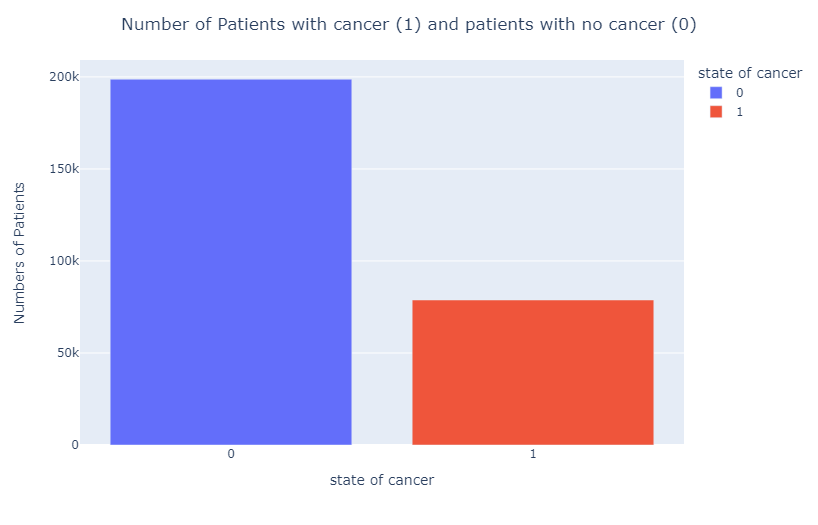
\includegraphics[width=0.7\textwidth]{Images/Histogram.png}
    \caption{Data distribution}
    \label{fig:Figure1}
\end{figure}
\begin{figure}[H]
    \centering
    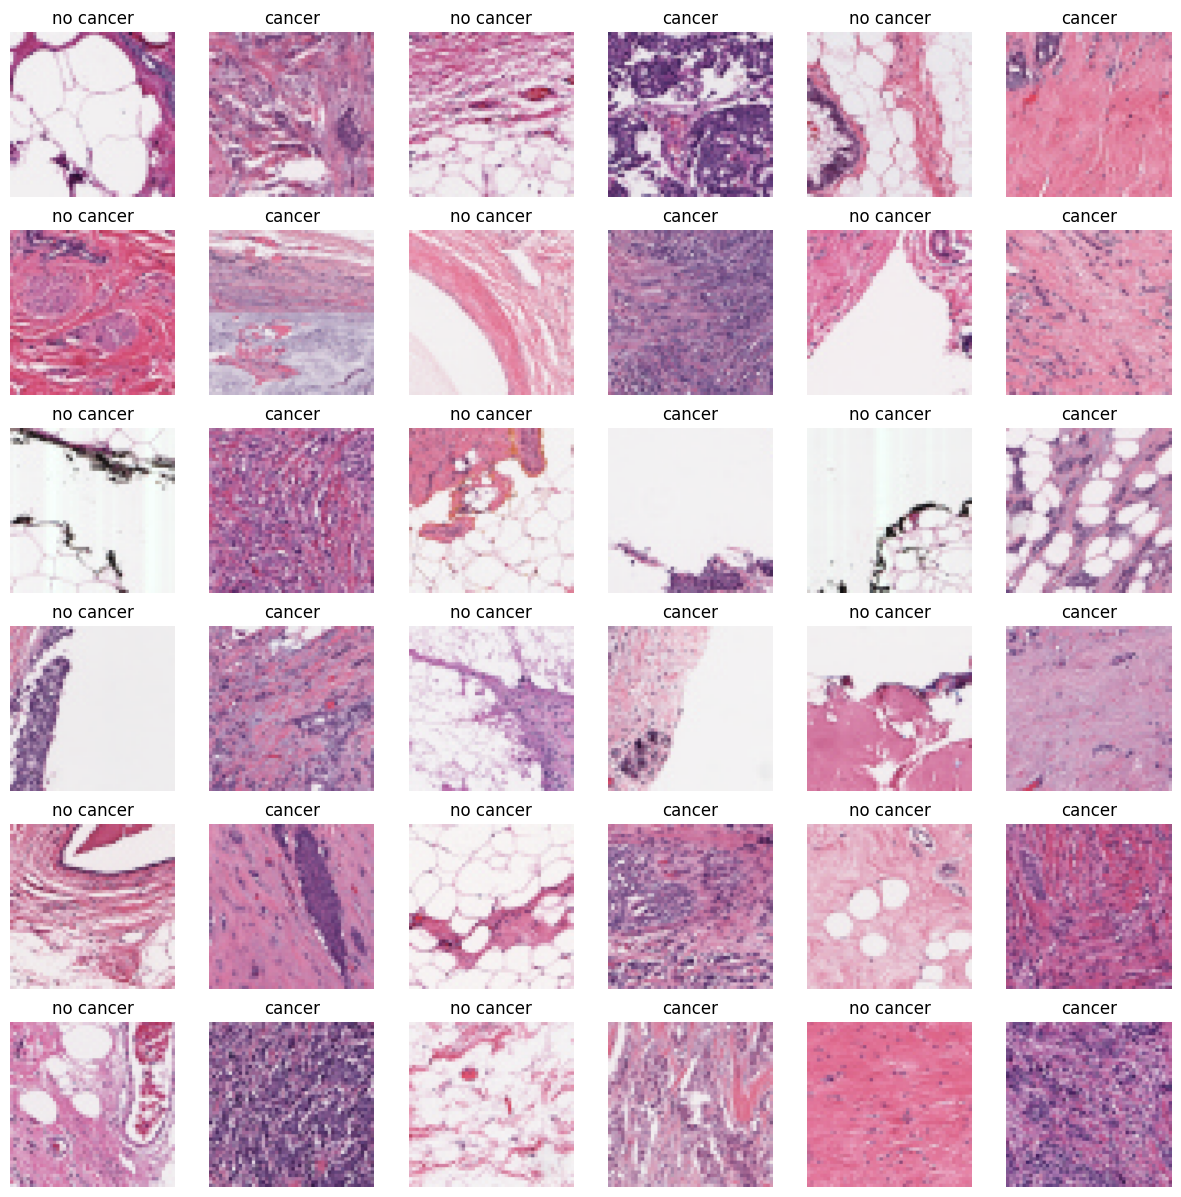
\includegraphics[width=0.5\textwidth]{Images/DataVisualization.png}
    \caption{Data Visualization}
    \label{fig:example}
\end{figure}
